\chapter{To POS Tag or Not to POS Tag: The Effect of POS Tags on Morphological Analysis in Low-Resource Settings}

\section{Abstract}

Part-of-Speech (POS) tags are routinely included as features in many NLP tasks. However, the importance and usefulness of POS tags needs to be examined as NLP expands to low-resource languages because linguists who provide many annotated resources do not place priority on early identification and tagging of POS. This paper describes an empirical study about the effect that POS tags have on two computational morphological tasks with the Transformer architecture. Each task is tested twice on identical data except for the presence/absence of POS tags, using published data in ten high- to low-resource languages or unpublished linguistic field data in five low-resource languages. We find that the presence or absence of POS tags does not have a significant bearing on performance. In joint segmentation and glossing, the largest average difference is an .09 improvement in F$_1$-scores by removing POS tags. In reinflection, the greatest average difference is 1.2\% in accuracy for published data and 5\% for unpublished and noisy field data.


\section{Introduction}
\label{sec:intro}


\begin{figure}
    \centering
    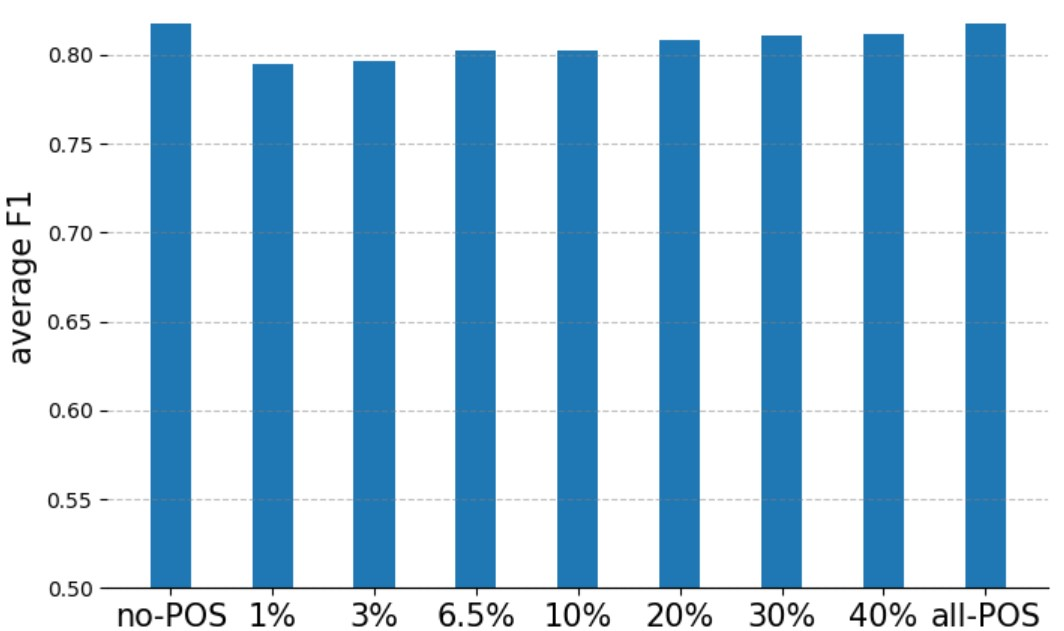
\includegraphics[width=20em]{figs/POS-avgSegGloss.jpg}
    \caption[POS Tags in Joint Segmentation and Glossing]{Joint segmentation and glossing on interlinear glossed texts from fieldwork in five languages found that increasing the percentage of tokens that are POS-tagged makes little difference in F$_1$-scores.}
    \label{fig:avgseggls}
\end{figure}

\begin{figure}
    \centering
    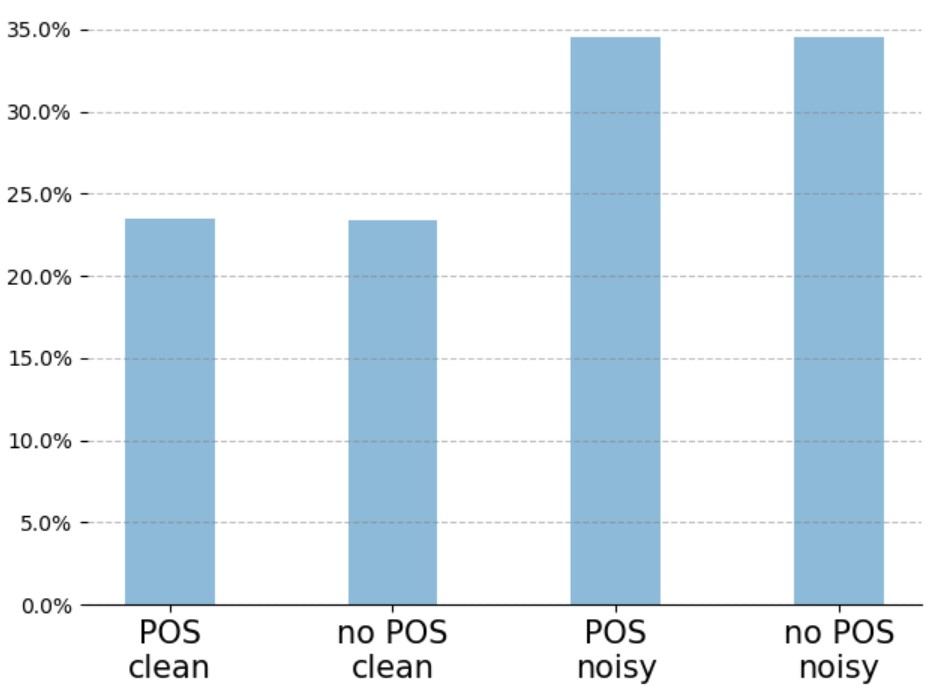
\includegraphics[width=25em]{figs/POS-avgReinfl.jpg}
    \caption[POS Tags in Reinflection of Noisy Data]{A reinflection task on four noisy field data corpora and four ``cleaned" versions found that the presence or absence of POS tags does not make a great difference in accuracy.}
    \label{fig:avgreinfl}
\end{figure}

Parts of speech (POS), also known as word classes or lexical categories, communicate information about a word, its morphological shape and inflectional paradigm, and its potential grammatical relations in a clause. POS have been used in work with many languages and POS tagging in NLP is a well-studied problem. POS tagging is one of the first tasks performed on a new data set and also one of the the first NLP tasks tackled in low-resource languages
\citep{yarowsky-ngai-2001-inducing,cox_probabilistic_2010,de_pauw_resource-light_2012,baldridge_learning_2013,duong_natural_2017,anastasopoulos_computational_2019,millour_unsupervised_2019,eskander_unsupervised_2020}. This priority on early POS tagging seems to reflect an long-held assumption that POS tags are helpful for other NLP work \citep{krauwer_basic_2003}. 
%POS tags have been claimed to play an important role in parsing, named entity recognition, co-reference resolution, and even disambiguating pronunciation in speech synthesis . 
As far as we are aware, this assumption has not been methodically tested. This paper describes an attempt to test the role of POS tags. 

When a sophisticated POS tagset and automatic POS taggers are available for a language and when there is no evidence that using POS tags are detrimental, the question of using POS tags may be a trivial one. However, as NLP expands into a broader range of languages, many of which are low-resource, the effect of POS tags needs to be tested because documentary and descriptive linguistics does not place as high a priority on POS tagging. Identifying what lexical categories exist in a language requires a detailed understanding of the language's syntax, which is something that linguists do not always possess in the early or intermediate stages of analysis. 
%Skimming through the head words of an English dictionary, for example, shows that parts of speech are not uniquely or consistently distinguished except for (most) adverbs which are marked with ``-ly''.
This means that unpublished linguistic field data often does not contain POS tags. A sufficient tag set may not even exist yet for a given language. Yet unpublished field data is often the largest available resource for a low-resource language. If POS tags are a necessary or important piece of information, then this common resource becomes less useful, but if POS tags do not have a significant effect, then effort could be shifted toward other, more fruitful research.

Testing the role of POS tags on all NLP tasks and their downstream effects is beyond the scope of one paper; we therefore focus on two related tasks in morphology. Both task involve morphological analysis---segmentation+glossing parses the morphological shape of words and reinflection generates inflected word forms. It is reasonable to expect that both tasks would benefit from POS tags, perhaps more than in other tasks, because of the morphosyntactic information conveyed by POS tags. POS tags might help segmentation algorithms distinguish affixes and glosses; for example, if a word is tagged as \textsc{verb}, then a final sequence ``ed'' is more likely to be a morpheme (that should be glossed `\textsc{past}'). This might, however, not hold true in languages where affixes are unambiguous (e.g. if ``ed'' rarely occurred word-finally on other lexical categories) or where ambiguous morphosyntactic features rarely occur by themselves (e.g. if plurality only appear with other nominal inflectional affixes).  Including POS tags could help reinflection tasks since, for example, morphemes that are otherwise identical (e.g. ``seat'') may use one set of inflectional morphemes as nouns (e.g. ``many seats'') and another as verbs (``be seated''). On the other hand, POS tags may be providing redundant information; for example where an affix that marks a certain inflected feature is identical across all categories where the feature appears (e.g. the Russian morpheme \textit{-i} `\textsc{pl}' is identical for plural nouns and plural verb agreement). 

The effect of POS tags on computational morphology may also hold implication for linguistic theory. 
%, although that is frequently lost in spoken language.
%, as we can see in phrases such as ``He works quick.'' 
The nature of lexical categories \citep{rauh_syntactic_2010}, the criteria for identifying them  \citep{croft_parts_2000}, and even their very existence as a universal property of language \citep{gil_word_2005} are not entirely settled among linguists. 
%For example, can words such as ``quick'', ``walk'', ``sleep'' in English be truly categorized as one particular category when they can function, without morphological change, as different categories within a sentence? And if lexical categories can only be determined in context,
If patterns of morphology can be analyzed and generated without reference to lexical categories, then perhaps such categories should not be considered an inherent property of the lexicon \citep{rauh_linguistic_2016}.

To test the assumption that POS tags are helpful, identical experiments were run that differed only in the presence or absence of POS tags, as illustrated in Figures \ref{fig:avgseggls} and \ref{fig:avgreinfl}. The results indicate that POS tags do not seem to give significant help in tasks relating to morphological analysis. Section \ref{sec:related} presents related work in POS-tagging, segmentation and glossing, and (re)inflection research. Sections \ref{sec:data} and \ref{sec:models} describe the data and models that are used in both tasks. The segmentation and glossing task and results are presented in Section \ref{sec:seggls}. The reinflection task and results are presented in Section \ref{sec:inflection}.  
%The implications of both studies are discussed in Section \ref{sec:discussion}.


\section{Related Work}
\label{sec:related}

Work on POS tagging has led to the development of several related resources in NLP and linguistics including numerous methods for automatic tagging (cf. \citet{KUPIEC1992225,toutanova2008a} among others) and tag sets. The most popular tag set for English was developed by the Penn Treebank Project \cite{penn_mitchell_1993}. A universal POS tag set was proposed by \cite{petrov-etal-2012-universal} and has been widely adopted in NLP. It closely follows traditional linguistic conventions for common lexical categories. In linguistics, the Leipzig Glossing Rules \citep{leipzig_glossing_rules} recommends tags for less common categories.

%\paragraph{Morpheme Segmentation and Glossing.}
Many NLP models have been applied to segmentation and glossing of low-resource languages, but the research often tackles just one of the two tasks. Automatic morpheme segmentation was introduced by \citet{harris_phoneme_1970} and much early segmentation research implemented unsupervised learning \cite{goldsmith_unsupervised_2001,creutz_unsupervised_2002,poon_unsupervised_2009}. Supervised models depend on annotated data provided by linguists and published data is usually used after some preprocessing in order to improve annotation quality. 
%\citet{moeller_automatic_2018} trained a joint segmentation and glossing system on Lezgi using field data.
Glossing-only experiments make the assumption that the data is already segmented into morphemes or that it does not need to be segmented. For example, \citet{mcmillan-major_automating_2020} trained a conditional random field (CRF) model to produce a gloss line for several high-resource languages and three low-resource languages. The low-resource language data came from interlinearized data and the data was first checked and polished for publication. McMillan-Major and some other experiments such as \citet{samardzic_automatic_2015} used information from other lines of interlinearized texts such as translation and POS tags.

%\paragraph{Morphological Inflection.} 
Computational approaches to morphological inflection or reinflection have been taken by \citet{durrett-denero-2013-supervised,nicolai-etal-2015-inflection,faruqui-etal-2016-morphological,kann-schutze-2016-single,aharoni-goldberg-2017-morphological}. Some of this work was developed as part of the SIGMORPHON Shared Tasks\footnote{https://sigmorphon.github.io/sharedtasks/} and our work replicates one of those tasks. Inflection models that perform well with limited data have been developed building on these earlier works \cite{kann-etal-2017-one,sharma-etal-2018-iit,makarov-clematide-2018-imitation,kann2020learning}, including systems developed by \newcite{wu-cotterell-2019-exact} and \newcite{wu2020applying} that have been successful in low-resource reinflection tasks.

\section{Data}
\label{sec:data}

We use published data in ten high- and low-resource languages and unpublished linguistic field data in five low-resource languages. Both joint segmentation+glossing and reinflection tasks use manually-annotated interlinear glossed text (IGT) from documentary and descriptive field projects. The morphological reinflection study uses the published data from the SIGMORPHON shared task.   


\subsection{SIGMORPHON Data}
\label{sec:sigdata}

For the morphological reinflection task we use datasets that were released for the CoNLL-SIGMORPHON 2018 shared task 1 \citep{cotterell-etal-2018-conll}. We selected 10 languages that belong to different families and are typologically diverse with regards to morphology. The languages and their parts-of-speech are listed in Table \ref{tab:SIGdata}. The language family and morphological typology for each language is available on the UniMorph official website.\footnote{\url{https://unimorph.github.io}} These languages are thoroughly and consistently POS-tagged and serve as a baseline for the reinflection task.  


\begin{table}
    \centering
    \begin{tabular}{lc}
        \textbf{Language} & \textbf{POS} \\
        \hline
        Adyghe  & N, ADJ \\
        Arabic & N, V, ADJ \\
        Basque & V \\
        Finnish & N, V, ADJ \\
        German & N, ADJ \\
        Persian & V \\
        Russian & N, V, ADJ \\
        Spanish & N, V \\
        Swahili & N, V, ADJ \\
        Turkish & N, V, ADJ \\
    \end{tabular}
    \caption{SIGMORPHON languages and the lexical categories found in the data.}
    \label{tab:SIGdata}
\end{table}


\subsection{Field Data}
\label{sec:igtdata}

\begin{table*}
    \centering
    \begin{tabular}{l|r|rc|c}
         \textbf{Language} & \textbf{Tokens} & \multicolumn{2}{c|}{\textbf{POS-tagged}}  & \textbf{Inflected}\\
         \hline
         Alas & 4.5k & 3845  & 86\% & 623 \\
         \hline
         Lamkang & 101k & 46,557 & 46\% & n/a \\
         \hline
         Lezgi & 14k & 13,636 & 96\%  & 843 \\
         \hline
         Manipuri & 12k & 2067 & 17\% & 3,260\\
         \hline
         Natügu & 16.5k & 10,994 & 66\% & 1,954\\
    \end{tabular}
    \caption{The approximate total number token counts in the field data does not include multiple-word-expressions (when parsed as such) and ignores personal nouns and digits. Only a percentage of total tokens are POS-tagged and their number is the amount of data available for segmentation/glossing. Of those the inflected words were usable for the reinflection.}
    \label{tab:IGTdata}
\end{table*}


The morpheme segmentation and glossing task only uses the IGT field data. This data is from low-resource and under-documented languages. Each corpus was compiled during a field project that had its own priorities and workflow and this resulted in differing amounts and types of annotation, as shown in Table \ref{tab:IGTdata}. Only POS-tagged words could be used in our studies and the amount of POS-tagged tokens is shown as a number and a percentage of the corpus. We used the POS tags provided by the annotators. For the reinflection task, the data was further limited to inflected forms. The collection of inflected forms have a clean and noisy version.
% Include this next line only if we also do morpheme POS comparison in seg/gloss experiment
%Four---Alas, Lezgi, Manipuri, and Nat\"ugu---IGT have a significant number of word-level POS tags and will be used in the inflection experiment. Arapaho and Tsez have ``POS'' tags only for morphemes and Lamkang has a very small amount of word-level POS tags, so these languages will be used only for the segmentation and glossing experiment.
%Less effort was made to represent various typological features, geographic areas, or language families. 
%The corpora were shared in the form of backup \texttt{flextext} XML files.\footnote{Rights holders gave informed consent to use the data for this research.}
It is worth noting that the Lamkang (used only for the segmentation and glossing study), Manipuri, and Nat\"ugu corpora are the result of many years of work. These extended projects eventually led to some POS tagging. Alas and Lezgi needed POS tags for specific research priorities and this led to early and more complete tagging. The Lezgi POS tags were annotated to help with research focusing on verb tenses in narrative discourse \citep{donet_importance_2014}. Many POS tags in the Lezgi corpus and all POS tags in the Alas corpus were added specifically for this research. 
%and other POS tags were added specifically for this project.
%Lamkang, is used only in the segmentation and glossing study.

\paragraph{Alas} 
[btz] (Alas-Kluet, Batak Alas, Batak Alas-Kluet) is an Austronesian language spoken by 200,000 people on the Indonesian island of Sumatra \cite{eberhard_ethnologue:2020}. Its morphology features reduplication, infixation, and circumfixation. The POS set in the corpus is: \textsc{\textbf{adj}, \textbf{adv}, aux, cardnum, clf, \textbf{conj}, cop, dem, distrnum, existmrkr, interj, \textbf{n}, nprop, ordnum, \textbf{prep}, \textbf{pro}, prt, quant, refl, relpro, \textbf{v}, vd, \textbf{vi}, \textbf{vt}}.\footnote{All POS were used for the segmentation and glossing task. Tags in boldface indicate POS that are inflected and were therefore used in the reinflection task.}
%POS tags found on inflected words are: \textsc{adj, adv, conj, n, prep, pro, v, vi, vt}. 

\paragraph{Lamkang} [lmk] is a Northern Kuki-Chin language of the Tibeto-Burman family with an estimated 4 to 10 thousand speakers primarily in Manipur, India but also in Burma \cite{lamkang_2007}. 
%Its endangerment status is not clear. 
Its morphology tends toward agglutination with many stem-stem patterns to signal syntactic categories. The corpus is accessible through the Computational Resources for South Asian Languages (CoRSAL) digital archive at the University of North Texas.\footnote{https://digital.library.unt.edu/explore/collections/SAALT/} The POS tag set is: \textsc{adn, advl, dem, conn, coordconn, cop, interj, n, npr, num, ordnum, postp, pron, ptc, quant, subo, unk,   v, vc, vi, vt}.

\paragraph{Lezgi} [lez] (Lezgian) is a highly agglutinative language belonging to the Lezgic branch of the Nakh-Daghestanian (Northeast Caucasian) family. It is spoken by over 400,000 speakers in Russia and Azerbaijan \cite{eberhard_ethnologue:2020}. It features overwhelmingly suffixing agglutinative morphology. The POS tag set is: \textsc{\textbf{adj}, \textbf{adv}, cardnum, conn, coordconn, \textbf{dem}, det, indfpro, interj, interrog, msd, multipnum, \textbf{n}, \textbf{nprop}, \textbf{num}, ordnum, \textbf{pers}, \textbf{poss}, post, prep, \textbf{pro}, proform, prt, ptcp, \textbf{recp}, subordconn, \textbf{v}, \textbf{verbprt}, \textbf{vf}, \textbf{vnf}, voc}.
% POS tags on inflected words: \textsc{adj, adv, dem, n, nprop, num, pers, poss, pro, proform, recp, v, verbprt, vf, vnf}.

\paragraph{Manipuri} [mni] (Meitei, Meetei) is a Tibeto-Burman language spoken by nearly two million people, primarily in the state of Manipur, and is one of India's official languages. It nonetheless has been classified as vulnerable to extinction \cite{moseley_atlas_2010}. It is a tonal language with weakly suffixing, agglutinative morphology \citep{Chelliah-1997}. The corpus is at CoRSAL.\footnote{\url{https://digital.library.unt.edu/explore/collections/MDR}} The POS set is: \textsc{\textbf{adv}, \textbf{interj}, \textbf{n}, \textbf{proform}, \textbf{unk}, \textbf{v}}. 
%for inflected word forms: \textsc{adv, interj, n, proform, v}.

\paragraph{Natügu} [ntu] belongs to the Reefs-Santa Cruz group in the Austronesian family and is spoken by about 4,000 people in the Temotu Province of the Solomon Islands. It has mainly agglutinative morphology with complex verb structures \cite{naess_ntu_2008}. The corpus is stored at SIL Language \& Culture Archives.\footnote{\url{https://www.sil.org/resources/search/language/ntu}} The POS tags set is: \textsc{\textbf{a-d-p2}, \textbf{adj}, \textbf{adv}, clause, \textbf{conj}, \textbf{dem}, \textbf{det}, \textbf{gen}, \textbf{gerund}, interrog, intj, \textbf{n}, \textbf{n.(kx.cl)}, ncomp, \textbf{neg}, \textbf{nom1}, np, np(comp), nprop, \textbf{num}, \textbf{ord}, \textbf{particle}, \textbf{pclf}, \textbf{perspro}, \textbf{phrase}, \textbf{pn}, \textbf{posspro}, \textbf{prep}, \textbf{pro}, \textbf{rprn}, \textbf{subr}, \textbf{unk}, \textbf{v}, \textbf{vi}, vp, \textbf{vt}, z-gerund}.
%for inflected words is: \textsc{a-d-p2, adj, adv, conj, dem, det, gen, gerund, n, n.(kx.cl), neg, nom1, num, ord, particle, pclf, perspro, phrase, pn, posspro, prep, pro, rprn, subr, unk, v, vi, vt} 

%\paragraph{Preprocessing Data.}
%First POS tag used for a word is added. Noisy IGT data may have several POS tags for a word.
%SIGMORPHON data only has inflected words. IGT data includes all words. 
%`~~~' and unk is used for untagged words. Not included
%


\section{Models}
\label{sec:models}

For simple comparions, we chose one neural model to train both tasks. All tasks were trained on the transformer model \citep{vaswani_attention_2017} for character-level transduction \citep{wu2020applying}, a state-of-the-art neural model for morphology learning in low-resource settings. We used the implementation of the Transformer model in the Fairseq toolkit \cite{ott-etal-2019-fairseq}.\footnote{\url{https://fairseq.readthedocs.io/en/latest/}} All models have been trained on an NVIDIA GP102[TITAN Xp] GPU
%We investigate the effect of POS tags with the following models from Section \ref{sec:models}: TODO


\section{POS for Segmentation and Glossing}
\label{sec:seggls}

We asked whether the presence/lack of POS tags makes a significant difference in an automated segmenting and glossing system. Our experiment compares the effect of POS tags when every word is tagged versus when no word is tagged. It also examines the benefit of tagging some of the words. 

Morpheme segmentation and glossing is an key task in early linguistic analysis. Once newly documented speech is transcribed, the next steps in linguistic analysis are to segment words into morphemes and gloss (strictly translate) those morphemes. This annotation is currently done primarily by hand which has caused an ``annotation bottleneck'' in the documentation and description of new languages \cite{simons_worlds_2013,holton_developing_2017,seifart_language_2018}. Automating this process could break the bottleneck. 
If POS tags make a significant positive difference to the task, they might be used to augment the input. 

\subsection{Experimental Setup}
\label{sec:segglssetup}

Three transformer models were trained for segmentation/glossing on all languages. Example (\ref{ex:POSSG}) uses a hypothetical English example to show how the models were trained. The input to the first model simulates data that has no POS tags, as shown in (\ref{ex:POSSG1in}). The second model includes a POS tag on every training example, as shown in (\ref{ex:POSSG23in}). The third model also includes POS tags, but only on some input examples.

\pex<POSSG>   
\label{ex:POSSG}
\a<a> \textbf{1 INPUT:} \hspace{2 mm} t \hspace{2 mm} a \hspace{2 mm} x \hspace{2 mm} e \hspace{2 mm} s 
\label{ex:POSSG1in}
\a<b> \textbf{2/3 INPUT:} \hspace{2 mm} t \hspace{2 mm} a \hspace{2 mm} x \hspace{2 mm} e \hspace{2 mm} s \hspace{2 mm} N
\label{ex:POSSG23in}
\a<c> \textbf{OUTPUT:} \hspace{2 mm} tax\#levy \hspace{2mm} -es\#\textsc{pl}
\label{ex:POSSGout}
\xe

Models 1 and 2 are trained on all the data as well as on differing amounts of training data. The training data was reduced to a percentage of the available data and gradually increased up to 40\%. We chose to focus our models on lower percentages in order to simulate various stages of the annotation process and test whether POS tags might be more helpful at the beginning stages. 

Even when POS tags are added to field data, the tagging is rarely complete, as  Table \ref{tab:IGTdata} clearly indicates.\footnote{This does not include two other large corpora which had no POS tags at all.}  
%Even when documentary corpora have some POS tags, it is not unusual for less than 50\% of the tokens in our corpus to be POS-tagged. 
We wanted to simulate a workflow where POS tags are added after segmentation/glossing is complete. Therefore, Model 3 was trained on all the data nine times but each time the percentage of tokens with POS tags was increased. We gradually added more POS tags to random training examples. For example, at 30\% one of three training examples have a POS tag. 
%This means every minute spent adding POS tags reduces time for more basic tasks. Therefore, we should not just ask if POS tags are beneficial, but also how much POS tagging is beneficial and at what point in the process of interlinearization should it become a focus. 

For all models, we wanted to simulate a situation where automated segmentation and glossing is being used to annotate more field data. In that situation, POS tags would not be available on the new data; therefore, the test sets do not include POS tags. The training/development/test split is 8/1/1 for all data sets. All the models are trained using a 10-fold cross-validation. The folds were trained twice, once with and once without POS tags; no other changes were made. All folds were evaluated on a single, consistent held-out dataset.
%Tables \ref{tab:POSSG} and \ref{tab:POSSGpsp} show the results of 10-fold averages.  

\subsection{Segmentation and Glossing Results}
\label{sec:segglsresults}

\begin{table*}
    \centering
    \begin{tabular}{l|cccccccc}
       %\textbf{Language} & 
       \textbf{Language} & \textbf{1\%} & \textbf{3\%} & \textbf{6.5\%} & \textbf{10\%} & \textbf{20\%} & \textbf{30\%} & \textbf{40\%} & \textbf{100\%} \\
       \hline
       %Alas 1 & \textbf{.0930} & \textbf{.2046} & \textbf{.3271} & \textbf{.3536} & \textbf{.5135} & \textbf{.5733} & \textbf{.6025} & \textbf{.6902} \\
       %Alas 2 & .0834 & .1814 & .3048 & .3277 & .4679 & .5260 & .5612 & .6968 \\
        Alas & .00 & .02 & .02 & .03 & .05 & .05 & .04 & -.09 \\
       %Alas delta & .0096 & .0232 & .0223 & .0259 & .0456 & .0473 & .0413 & .0944 \\
       \hline
       %Lamkang 1 & .3059 & .5064 & .6481 & .6820 & .7783 & .8077 & .8273 & .8573  \\
       %Lamkang 2 & .2512 & .4279 & .5744 & .6090 & .6958 & .7268 & .7518 & 0.8645 \\
       %Lamkang delta & .0547 & .0785 & .0737 & .0730 & .0825 & .0809 & .0757 & -.0072 \\
       Lamkang & .05 & .08 & .07 & .07 & .08 & .08 & .08 & -.01 \\
       \hline
       %Lezgi 1  & \textbf{.2262} & \textbf{.3077} & \textbf{.4410} & \textbf{.4729} & \textbf{.6391} & \textbf{.6679} 
       %Lezgi 2 & .1998 & .3150 & .4207 & .4294 & .6137 & .6388 & .6670 & .7317  \\
       %Lezgi delta & .0264 & -.0050 & .0203 & .0435 & .0254 & .0291 & .0279 & .0184 \\
       Lezgi & .03 & -.01 & .02 & .04 & .03 & .03 & .03 & .02 \\
       \hline
       %Manipuri 1 & .1971 & \textbf{.3976} & .5795 & .6162 & .7632 &  &  & .8903 \\
       %Manipuri 2 & \textbf{.2036} & .3932 & .5733 & .6139 & .7618 & .8086 & .8325 & \textbf{.8921}  \\
       %Manipuri delta & -.0065 & .0044 & .0062 & .0023 & .0014 & .0050 & .0038 & -.0018 \\
       Manipuri & -.01 & .00 & .01 & .00 & .00 & .01 & .00 & .00 \\
       \hline
       %Nat\"ugu 1 & \textbf{.2405} & \textbf{.4747} & \textbf{.6162} & \textbf{.6466} & \textbf{.7617} &  &  &  .8995 \\
       %Nat\"ugu 2 & .2352 & .4423 & .5915 & .6182 & .7408 & .7708 & .8012 & \textbf{.9006}  \\
       %  & 0.0 & 0.0 & 0.0 & 0.0 & 0.0 & .7708 & .8012 & 0.0 \\
       %Nat\"ugu delta & .0053 & .0324 & .0249 & .0284 & .0209 & .0417 & .0377 & -.0011 \\
       Nat\"ugu & .01 & .03 & .02 & .03 & .02 & .03 & .04 & .00 \\
    \end{tabular}
    \caption[Segmenting and Glossing with/out POS tags]{The difference in F$_1$ scores with/out POS tags when training segmentation and glossing on increasing amounts of annotated data, as percentages of total available data. Negative scores indicates that adding POS tags improve results.
    %(pos) and morpheme-level ``POS'' tags (mpos).
    }
    \label{tab:POSSG}
\end{table*}


The effect made by the presence or absence of POS tags is slight or negligible. The presence of POS tags has no clear positive effect in these low-resource settings. Table \ref{tab:POSSG} shows the differences between F$_1$-scores when training with and without POS tags using various amounts of training data. To determine the effect that POS tags have, the results with POS tags were subtracted from the results without POS tags. The difference between the two is never more than .1 points. Manipuri, which shows the smallest difference, has the smallest amount of POS-tagged data, and also the smallest POS set by far. The largest differences is in Alas and Lamkang. Like Manipuri, Alas has a small data set, but it has quite a large POS set. As the amount of Alas grows, the effect of POS tags becomes more pronounced, suggesting that a relatively large POS tag set may have a greater effect on results. Lamkang has the largest POS-tagged data set, but a significant number of tokens were tagged as \textsc{unk}. It is not clear whether the \textsc{unk} tag is limited to certain categories that have not been fully analyzed or if it is a default tag that covers a diverse set of words. The difference made by adding POS tags all but disappears when all Lamkang data is added, suggesting that a large data set may be less likely to be overwhelmed by a large POS or inconsistent tag set.


\begin{table*}[]
    \centering
    \begin{tabular}{l|ccccccccc}
       %\textbf{Language} & 
       \textbf{Language} & \textbf{0\%} & \textbf{1\%} & \textbf{3\%} & \textbf{6.5\%} & \textbf{10\%} & \textbf{20\%} & \textbf{30\%} & \textbf{40\%} & \textbf{100\%}  \\
       \hline
       Alas  & .6902 & .6448  & .6415 & .6546 & .6517 & .6627 & .6647 & .6708 & \textbf{.6968} \\
       \hline
       Lamkang & .8573 & .8074 & .8195 & .8298 & .8332 & .8482 & .8527 & .8524 & \textbf{.8645}  \\
       \hline
       Lezgi  & .7501 & \textbf{.7564} & .7542 & .7529 & .7505 & .7498 & .7480  & .7471 & .7317 \\
       \hline
       Manipuri & .8903 & .8885 & .8877 & .8882 & .8889 & .8874 & .8896 & .8897 & \textbf{.8921} \\
       \hline
       Nat\"ugu & .8995 & .8748 & .8782 & .8864 & .8855 & .8932 & .8999 & .8965 & \textbf{.9006} \\
    \end{tabular}
    \caption{F$_1$ scores on segmenting and glossing when trained on all data with increasing percentages of POS tags.}
    \label{tab:POSSGpsp}
\end{table*}

Table \ref{tab:POSSGpsp} shows the F$_1$-scores when all data is used for training but the amount of POS tags in the data is gradually increased. Overall, increasing the number of POS tags has minimal effect on the results. The greatest improvement that can be made by adding any amount of POS tags is .0072 in F$_1$-scores (Lamkang). In most cases having partially complete POS tags is worse than having none at all. When only a few words have POS tags, the system either performs worse than when having no POS tags, or, in the case of Lezgi, makes very small improvement (.0066 points). Except for Lezgi, as more POS tags are added, the system tends to improves slightly. It is not clear why Lezgi differs from the other data sets, but it is known that this data was POS-tagged by multiple people who may have applied different analyses when identifying lexical categories.


\section{POS for Reinflection}
\label{sec:inflection}

This section asks whether the presence or absence of POS tags make a significant difference to learning a language's morphological paradigms. Once a newly documented language has a sufficient amount of segmented and glossed data, a common next step is determining the language's patterns of morphological inflection. The pattern of inflection for a given word or lexical category, including all possible inflected forms, is its morphological paradigm. Learning morphological paradigms from data can be cast in terms of filling the missing forms in a paradigm table, that is, correctly generating inflected forms that are not attested in the data. 

We test whether the presence/lack of POS tags has significant effect on learning a languages' morphological patterns by replicating a SIGMORPHON reinflection task on three sets of data. The task of morphological reinflection consists of generating unknown inflected forms, given an inflected form 
$f(\ell, \vec{t}_{\gamma_1})$ and a target feature vector $\vec{t}_{\gamma_2}$. Thus, it corresponds to learning the mapping $f : \Sigma^* \times \mathcal{T} \to \Sigma^*$. The goal is then to produce the inflected form $f(\ell, \vec{t}_{\gamma_2})$.
%One task that replicate this is the SIGMORPHON's reinflection task, where an unseen inflected form is generated when given another related form and the morphosyntactic features of the target form. 
In previous reinflection work, POS tags were included by default as part of the morphological features.


\subsection{Experimental Setup}
\label{sec:inflectionsetup}

First, we test on published data in ten languages and then on unpublished field data in four languages. This data can be viewed as three groups with different amounts of preprocessing. The SIGMORPHON data was extracted from published data and is the ``cleanest''. Its inflected forms and morphological features were double-checked and the forms provided were chosen to provide a balanced picture of the language's morphological structure. The field data was extracted directly from the interlinear glossed text and contains only the inflected forms attested in those examples of natural speech. It has a clean and noisy version. The noisy version was automatically grouped into paradigms based on the assumption that identical glosses of root morphemes signified the same lemma, and therefore the same morphological paradigm. The clean data was created by language experts who examined the noisy data and regrouped paradigms when root morphemes were incorrectly glossed; they also corrected typos and morphological features. 

For the curated data, the original SIGMORPHON training/validation/test splits were kept but only the \textit{medium} setting of 1,000 training examples were used. Using 1,000 training examples is the closest size to the the other four data sets. The field data provided between 600 and 3,000 training examples. 


\subsection{Reinflection Results}
\label{sec:inflectionresults}

\begin{figure*}[t]
    \centering
    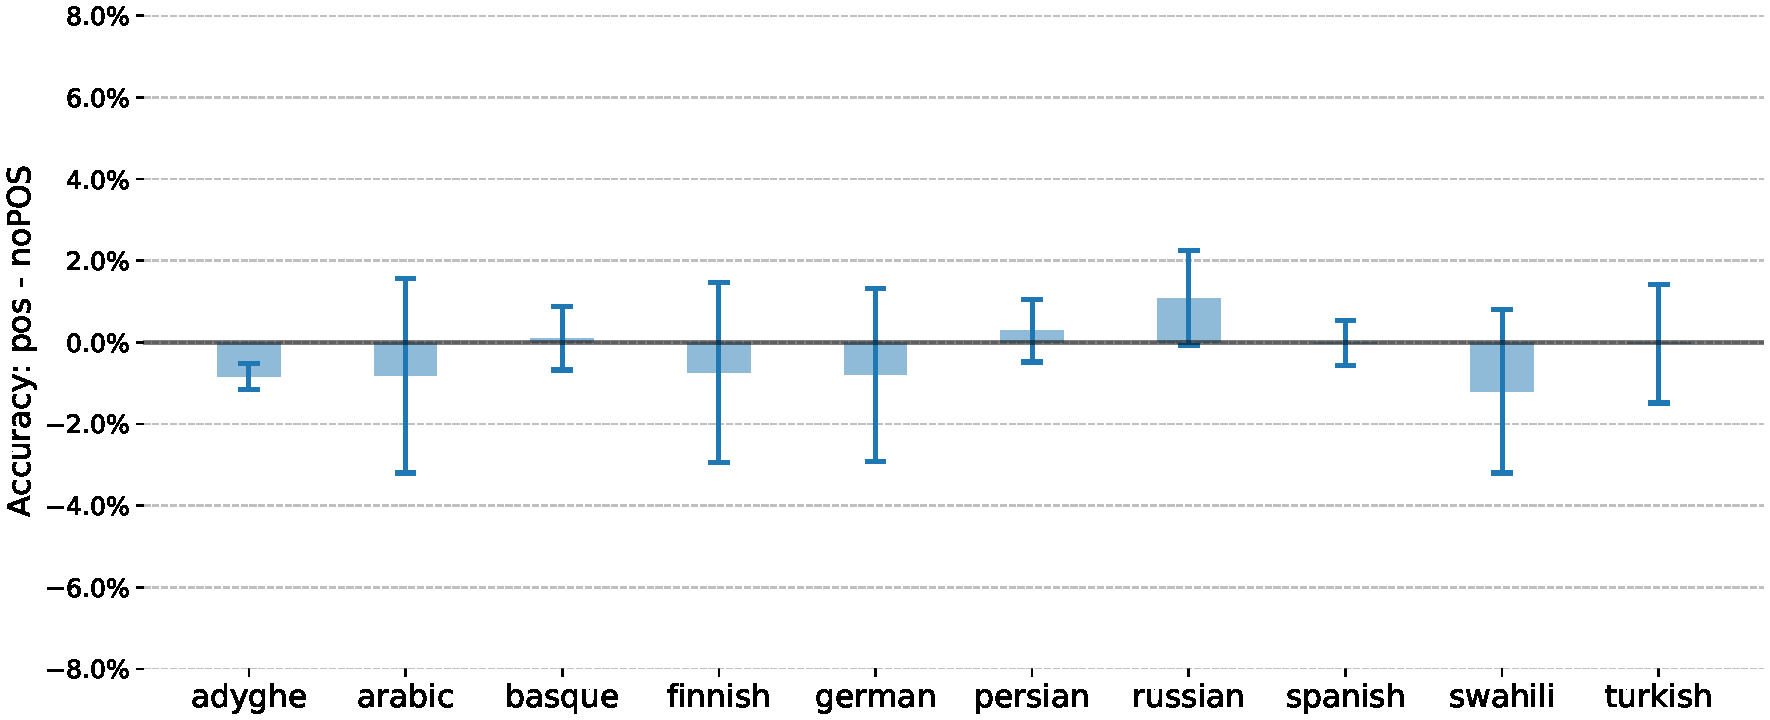
\includegraphics[width=35em]{figs/plot_2018data.pdf}
    \caption{The difference in accuracy with/out POS on the reinflection task with SIGMORPHON languages. Negative scores indicates that removing POS tags improves results. The bar shows the mean of the differences and lines indicate the range of the mean plus or minus the standard deviation.}
    \label{fig:sigreinfl}
\end{figure*}

\begin{figure*}[t]
    \centering
    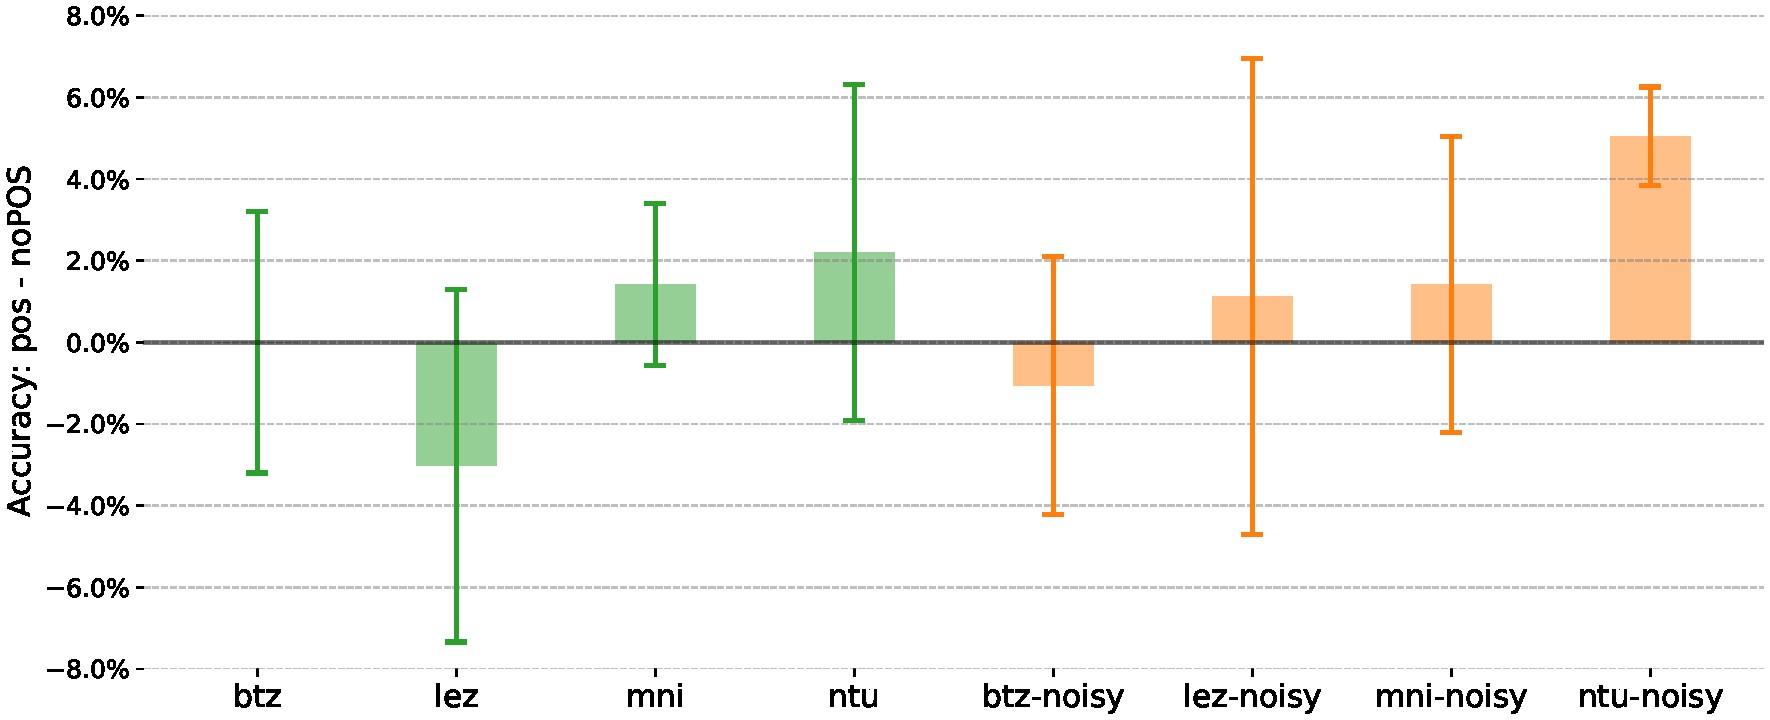
\includegraphics[width=41em]{figs/plot_igtdata.pdf}
    \caption{The difference in accuracy with/out POS on the reinflection task with cleaned and noisy field data. Negative scores indicates that removing POS tags improve results. The bar shows the mean of the differences and line indicates the range of the mean plus or minus the standard deviation.}
    \label{fig:igtreinfl}
\end{figure*}

Figures \ref{fig:sigreinfl} and \ref{fig:igtreinfl} show the differences in accuracy when including and not including POS tags in the reinflection task. Five models were run with random seeds. All models are trained twice, once with and once without POS tags on the input. Crosswise pairs were compared by subtracting the results without POS tags from the results with POS, giving 25 scores per language. 

The range of differences shows that the presence or absence of POS tags does not have a clear positive or negative effect. Only two languages show a consistent effect either way. In Nat\"ugu, the presence of POS tags improves results. In Adyghe, the presence of POS tags decreases accuracy.

%(see Table \ref{tab:pos-acc-detail} in the appendix for accuracy details). 
The average difference for any language is rarely more than 1 percentage point in accuracy. As the data becomes less polished and more noisy, the average effect of POS tags increases slightly and the range of differences grows noticeably. For the SIGMORPHON languages the largest mean difference is barely over 2 points. For the clean field data, the largest mean difference is about 3 points of higher accuracy \textit{without} POS tags. The noisy field data shows the greatest and largest range of differences, with the highest average difference reaching about 5 points decreased performance \textit{with} POS tags in the noisy Nat\"ugu [ntu] data.


%The Lezgi data presents an anomaly among the field data sets because it is the only where accuracy reduces on the clean data. There was significant variation in accuracy across the five models of the Lezgi clean data without POS tags. This may indicate that POS tags might sometimes be helpful for this heavily agglutinative language, but the difference is not large enough to say this with certainty and the test should be repeated on related Nakh-Daghestanian languages.
%LOOK AT LEZGI DATA


\section{Discussion}

The sample of language used for our studies is small but a few observations can be made which should be tested in future work on a broader range of languages.

For both tasks the effect made by the presence of absence of POS tags is minimal. There is no clear advantage to having POS tags. Some of the largest differences were an improvement made by removing POS tags. In general, it seems that having more POS tags in a corpus is better having only a few, but best results in a small corpus are achieved when either all or no tokens are POS-tagged. 

The size of the tag set may make a difference in the effect that POS tags have. When comparing the tag sets in the SIGMORPHON data and the POS tag found in the interlinear gloss texts from fieldwork, the number of tags is noticeable. The SIGMORPHON data sets are limited to noun (\textsc{n}), verb (\textsc{v}), and adjective (\textsc{adj}) at most. Field data, by contrast, includes far more POS tags. The six POS tags that Manipuri uses is already twice as many POS tags as the SIGMORPHON languages but the set is much smaller than the other languages, all of which have over 20 unique labels in their tagset. These tags are very specific labels for lexical categories and illustrate the focus on descriptive work where, for example a finite verb form (\textsc{vf}) is distinguished from a non-finite form (\textsc{vnf}. Descriptive labels may represent distinct lexical categories in a language, but may also simply indicate specific inflectional or derivational forms or reflect semantic classes with no morphological differences, like proper nouns (\textsc{nprop} and common nouns in English. 
Re-tagging the field data using more general tags may change the results. However, the overall effect of POS tags on these languages is not significantly different from SIGMORPHON languages which do have generalized tag sets.

%The tag sets provided by annotators in the field data included tags such as <NotSure> or <AttachesToAnyCategory>. This means that less POS tags are actually available than shown in Table \ref{tab:data}. What happens if filtered?

In the reinflection task, the range of average effect made by the presence or absence of POS tags is larger with unpublished data and the largest range and average difference is found in the noisy unpublished data. Future work should investigate what what factors lend to this range of difference and how they could be minimized. %Consistency of annotation may be significant. Metrics for annotation quality should be devised so that . Linguists need to know what as they start what is important to focus on in order to gain best automated help later. 

\section{Conclusion}

We conclude that the presence or absence of POS tags does not make a significant difference in two morphological analysis tasks: segmentation and glossing, or reinflection. In segmentation and glossing, the greatest average difference is a loss of .09 F$_1$-score when a large POS tag set is added to a small field corpus. In the reinflection task, the overall tendency, though slight, is that accuracy decreases when POS tags are added. The greatest average effect is 1.2 percentage points of accuracy for published data, 2.2 points for unpublished preprocessed data, and 5 points for unpublished noisy field data.

We hypothesize that POS tags do not have a significant effect because the information provided by POS tags may be implicitly learned. These are only two tasks where POS tags could have an effect on results and our results do not warrant a definitive statement regarding the usefulness of POS tags in other tasks, but it does bring into question whether POS tagging and the development of POS taggers should be given early priority when working with low-resource languages. The results suggest that the usefulness of POS tags needs further testing and justification. Future work should explore what other tasks could benefit from inclusion or exclusion of POS tags as the answer may affect annotation priorities when working with low-resource languages.

%If POS tags are not helpful in learning morphological patterns, what does this mean for questions about POS being a universal property of language?

%Testing the assumption that POS tags are useful in low-resource settings is an interesting question because documentary and descriptive linguistics, which create annotated resources in new languages, does not put as high a priority on identifying lexical categories as NLP does. 
%POS-tagging is rarely, if ever, mentioned as part of the language documentation workflow 
%and if POS tagging is prioritized, then it is usually because the project's short-term goals will directly benefit from it, such as allowing descriptive work to focus on verb tenses in narrative discourse.
%For example, a linguist studying the salience of verb tenses in narrative discourse may prioritize lexical categories identification so that early analytic tasks such as morpheme segmentation and glossing can be focused on the verbs. 
%Several other tasks are prioritized over POS tagging, including translation, morpheme segmentation and glossing, lexicon building, morphological inflectional paradigm elicitation, and even sketching a full grammar \cite{bird_machine_2012}. This mismatch of priorities presents a potential conflict for NLP work with low-resource languages or for leveraging NLP systems to assist linguistic analysis of under-documented languages. 
%, even a similar tagging process for morphemes (not words) .
%which is similar to POS tagging but tags morphemes, not words. Without a good knowledge of the language's structure, it may not be possible to decipher POS information from the morpheme tags.  

%It makes little sense to introduce one more task to already overburdened field linguists if the task holds little promise to improve or speed their later work or the development of NLP. This is particularly weighty when we consider how complicated the task can be. 
 
